\section{Systemarkitektur}
\label{chap:systemarkitektur}

Til at dokumentere systemarkitekturen er der anvendt SysML og UML diagrammer. SysML diagrammer har beskrevet hardware moduler hvor UML diagrammerne har stået af systemets software del.

Nedenfor kommer en beskrivelse af de SysML diagrammer der er anvendt i projektet. UML diagrammer bliver beskrevet i kapitel

\subsection{Blokbeskrivelser}
Det overordnede bdd på figur \ref{fig:bdd_asd} viser hvilke blokke systemet består af, samt hvilke parts blokkene indeholder.

\begin{figure}[H]
	\centering
	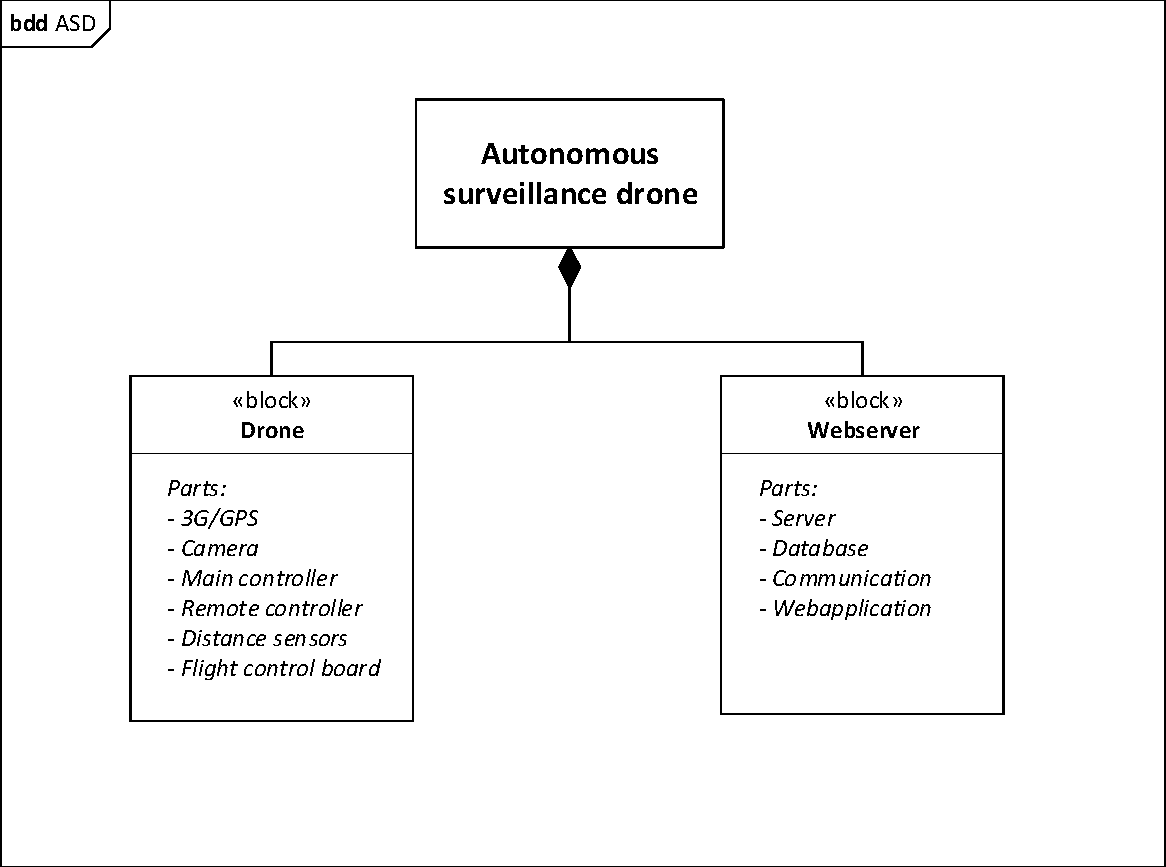
\includegraphics[width=0.80\textwidth]{Billeder/Projektbeskrivelse/bdd_overordnet.pdf}
	\caption{Overordnet bdd for systemet}
	\label{fig:bdd_asd}
\end{figure}

\textbf{Drone} \\


\textbf{Webserver} \\



\subsection{Interne forbindelser}

Det overordnede ibd på figur \ref{fig:ibd_asd} beskriver hvorledes de forskellige blokke kommunikerer samt hvilken type signal, der anvendes.

\begin{figure}[H]
	\centering
	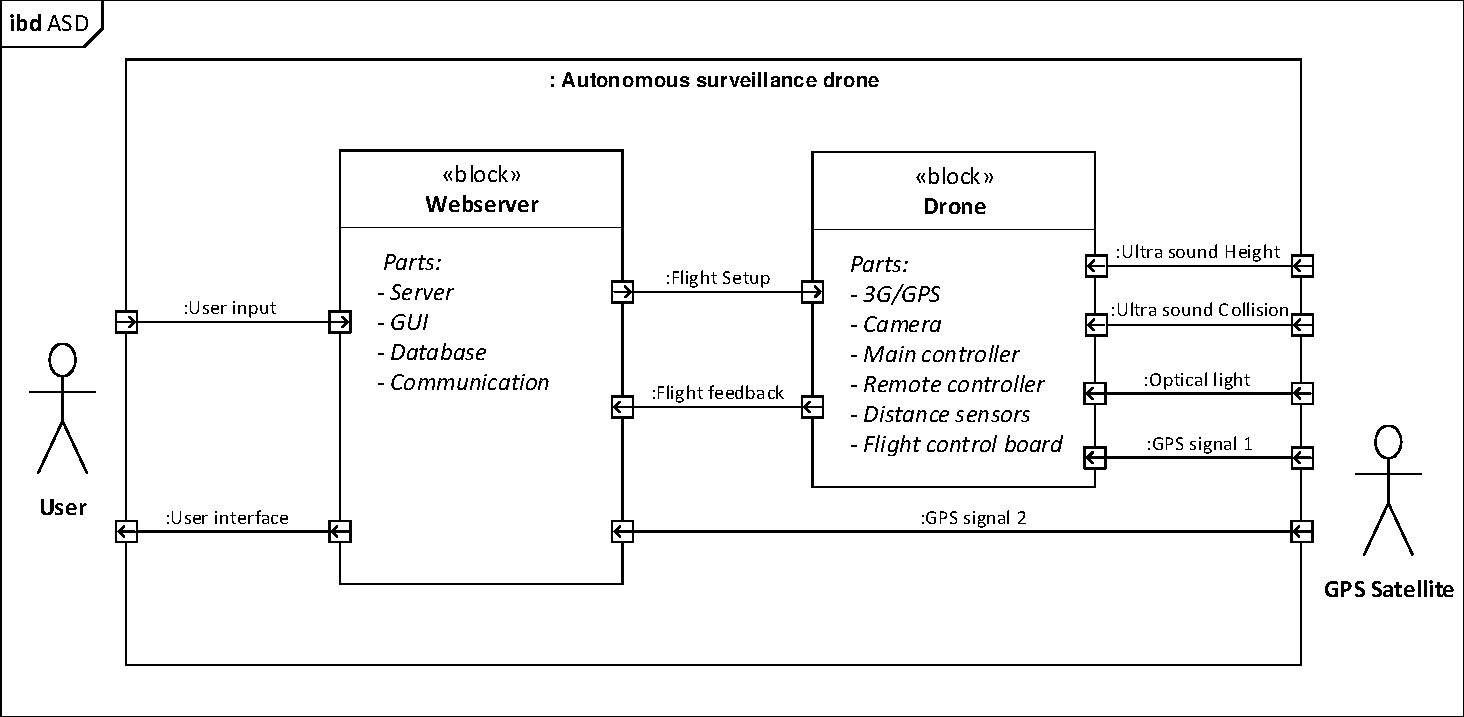
\includegraphics[width=1\textwidth]{Billeder/Projektbeskrivelse/ibd1_overordnet.pdf}
	\caption{Overordnet ibd for systemet}
	\label{fig:ibd_asd}
\end{figure}




\subsection{•}